\begin{song}{title=\centering Nagasaki Hirošima \\\normalsize Mňága \&  Žďorp  \vspace*{-0.3cm}}  %% sem se napíše jméno songu a autor
\moveright 4.5cm \vbox{      %Varianta č. 1  ---> Jeden sloupec zarovnaný na střed	

\sloka
	^{A{\color{white}\_\_\_}}Tramvají ^{E{\color{white}\_\_\_}}dvojkou ^{D{\color{white}\_\_\_}}jezdíval ^{E}jsem do ^{{\color{white}\_}\,A}Židenic, ^{E\,\,D\,\,E}

	z ^{A}tak velký ^{E{\color{white}\_\_}}lásky ^{D{\color{white}\_\_\_}}většinou ^{E{\color{white}\_\_\_}}nezbyde ^{F#mi}nic.

	Z ^{D\,{\color{white}\_\_}}takový ^{A\,{\color{white}\_}}lásky ^{D{\color{white}\_}}jsou kruhy ^{A{\color{white}\_}}pod ^{{\color{white}\_}E}očima

	a dvě ^{A{\color{white}\_\_\_}}spálený ^{E{\color{white}\_\_}}srdce -- ^{D\,\,{\color{white}\_\_\_}}Nagasaki ^{E\,\,{\color{white}\_\_\_}}Hirošima. ^{A\,\,E\,\,D\,\,E}

\sloka
	Jsou jistý věci, co bych tesal do kamene,
	
	tam, kde je láska, tam je všechno dovolené
	
	a tam, kde není, tam mě to nezajímá.
	
	Jó dvě spálený srdce Nagasaki Hirošima.

\sloka
	Já nejsem svatej, ani ty nejsi svatá,
	
	jablka z ráje bejvala jedovatá,
	
	jenže hezky jsi hřála, když mi někdy byla zima.
	
	Jó dvě spálený srdce Nagasaki Hirošima.

\sloka
	Tramvají dvojkou jezdíval jsem do Židenic,
	
	z takový lásky většinou nezbyde nic.
	
	Z takový lásky jsou kruhy pod očima

	/: a dvě spálený srdce Nagasaki Hirošma. :/
	
	/: A dvě spálený srdce Nagasaki Hirošma. :/


}
\setcounter{Slokočet}{0}
\end{song}


\begin{figure}[h]
\centering
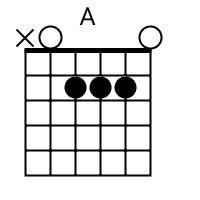
\includegraphics[width=3cm]{../Akordy/a.png}
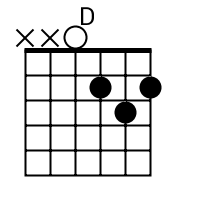
\includegraphics[width=3cm]{../Akordy/d.png}
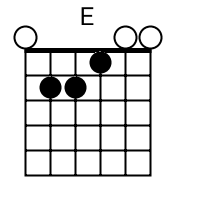
\includegraphics[width=3cm]{../Akordy/e.png}
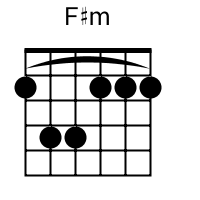
\includegraphics[width=3cm]{../Akordy/fxm.png}
\end{figure}
